\chapter{Introduction}

\section{Background}
During the spring of 2013 BorgWarner AB went into production with their new product called Front Cross Differential (FXD). This is a brand new electronic Limited Slip Differential (eLSD) for front wheel driven cars which uses some of the technology from their well known four wheel drive systems. Being able to control the applied torque on each wheel results in increased traction, better cornering performance and improved safety.

The torque control is done by a complex algorithm that uses several signals from the car. It has been shown that the tuning of this algorithm is different depending on tire stiffness and road condition. It is therefore desirable to extend the algorithm to be able to estimate tire stiffness and the tire/road friction coefficient.

\section{Project goal}
The goal of the project is to estimate the tire stiffness and the tire/road friction coefficient. The system needs to be fast and robust to be trusted in all conditions. Another constraint is to make an estimator that relies on signals easily available on the Controller Area Network (CAN) bus of the vehicle. It's supposed to work in a normal car and not only be restricted to testing in cars equipped with advanced technology to measure signals that's not normally available. 

\section{Volkswagen Golf GTi Mk7}
The latest Golf GTi from Volkswagen is equipped with the FXD. All driving data used in this work have been collected with this kind of car. Borg Warner has one of these cars in Landskrona that has been driven to collect data. The car at Borg Warner is equipped with Volkswagens DSG transmission which is an automatic transmission with the options to shift gear manually with paddles at the steering wheel. At all time in the report when a car is referred to, it is this Golf GTi, if nothing else is explicitly stated.

\begin{figure}[h]
	\centering
	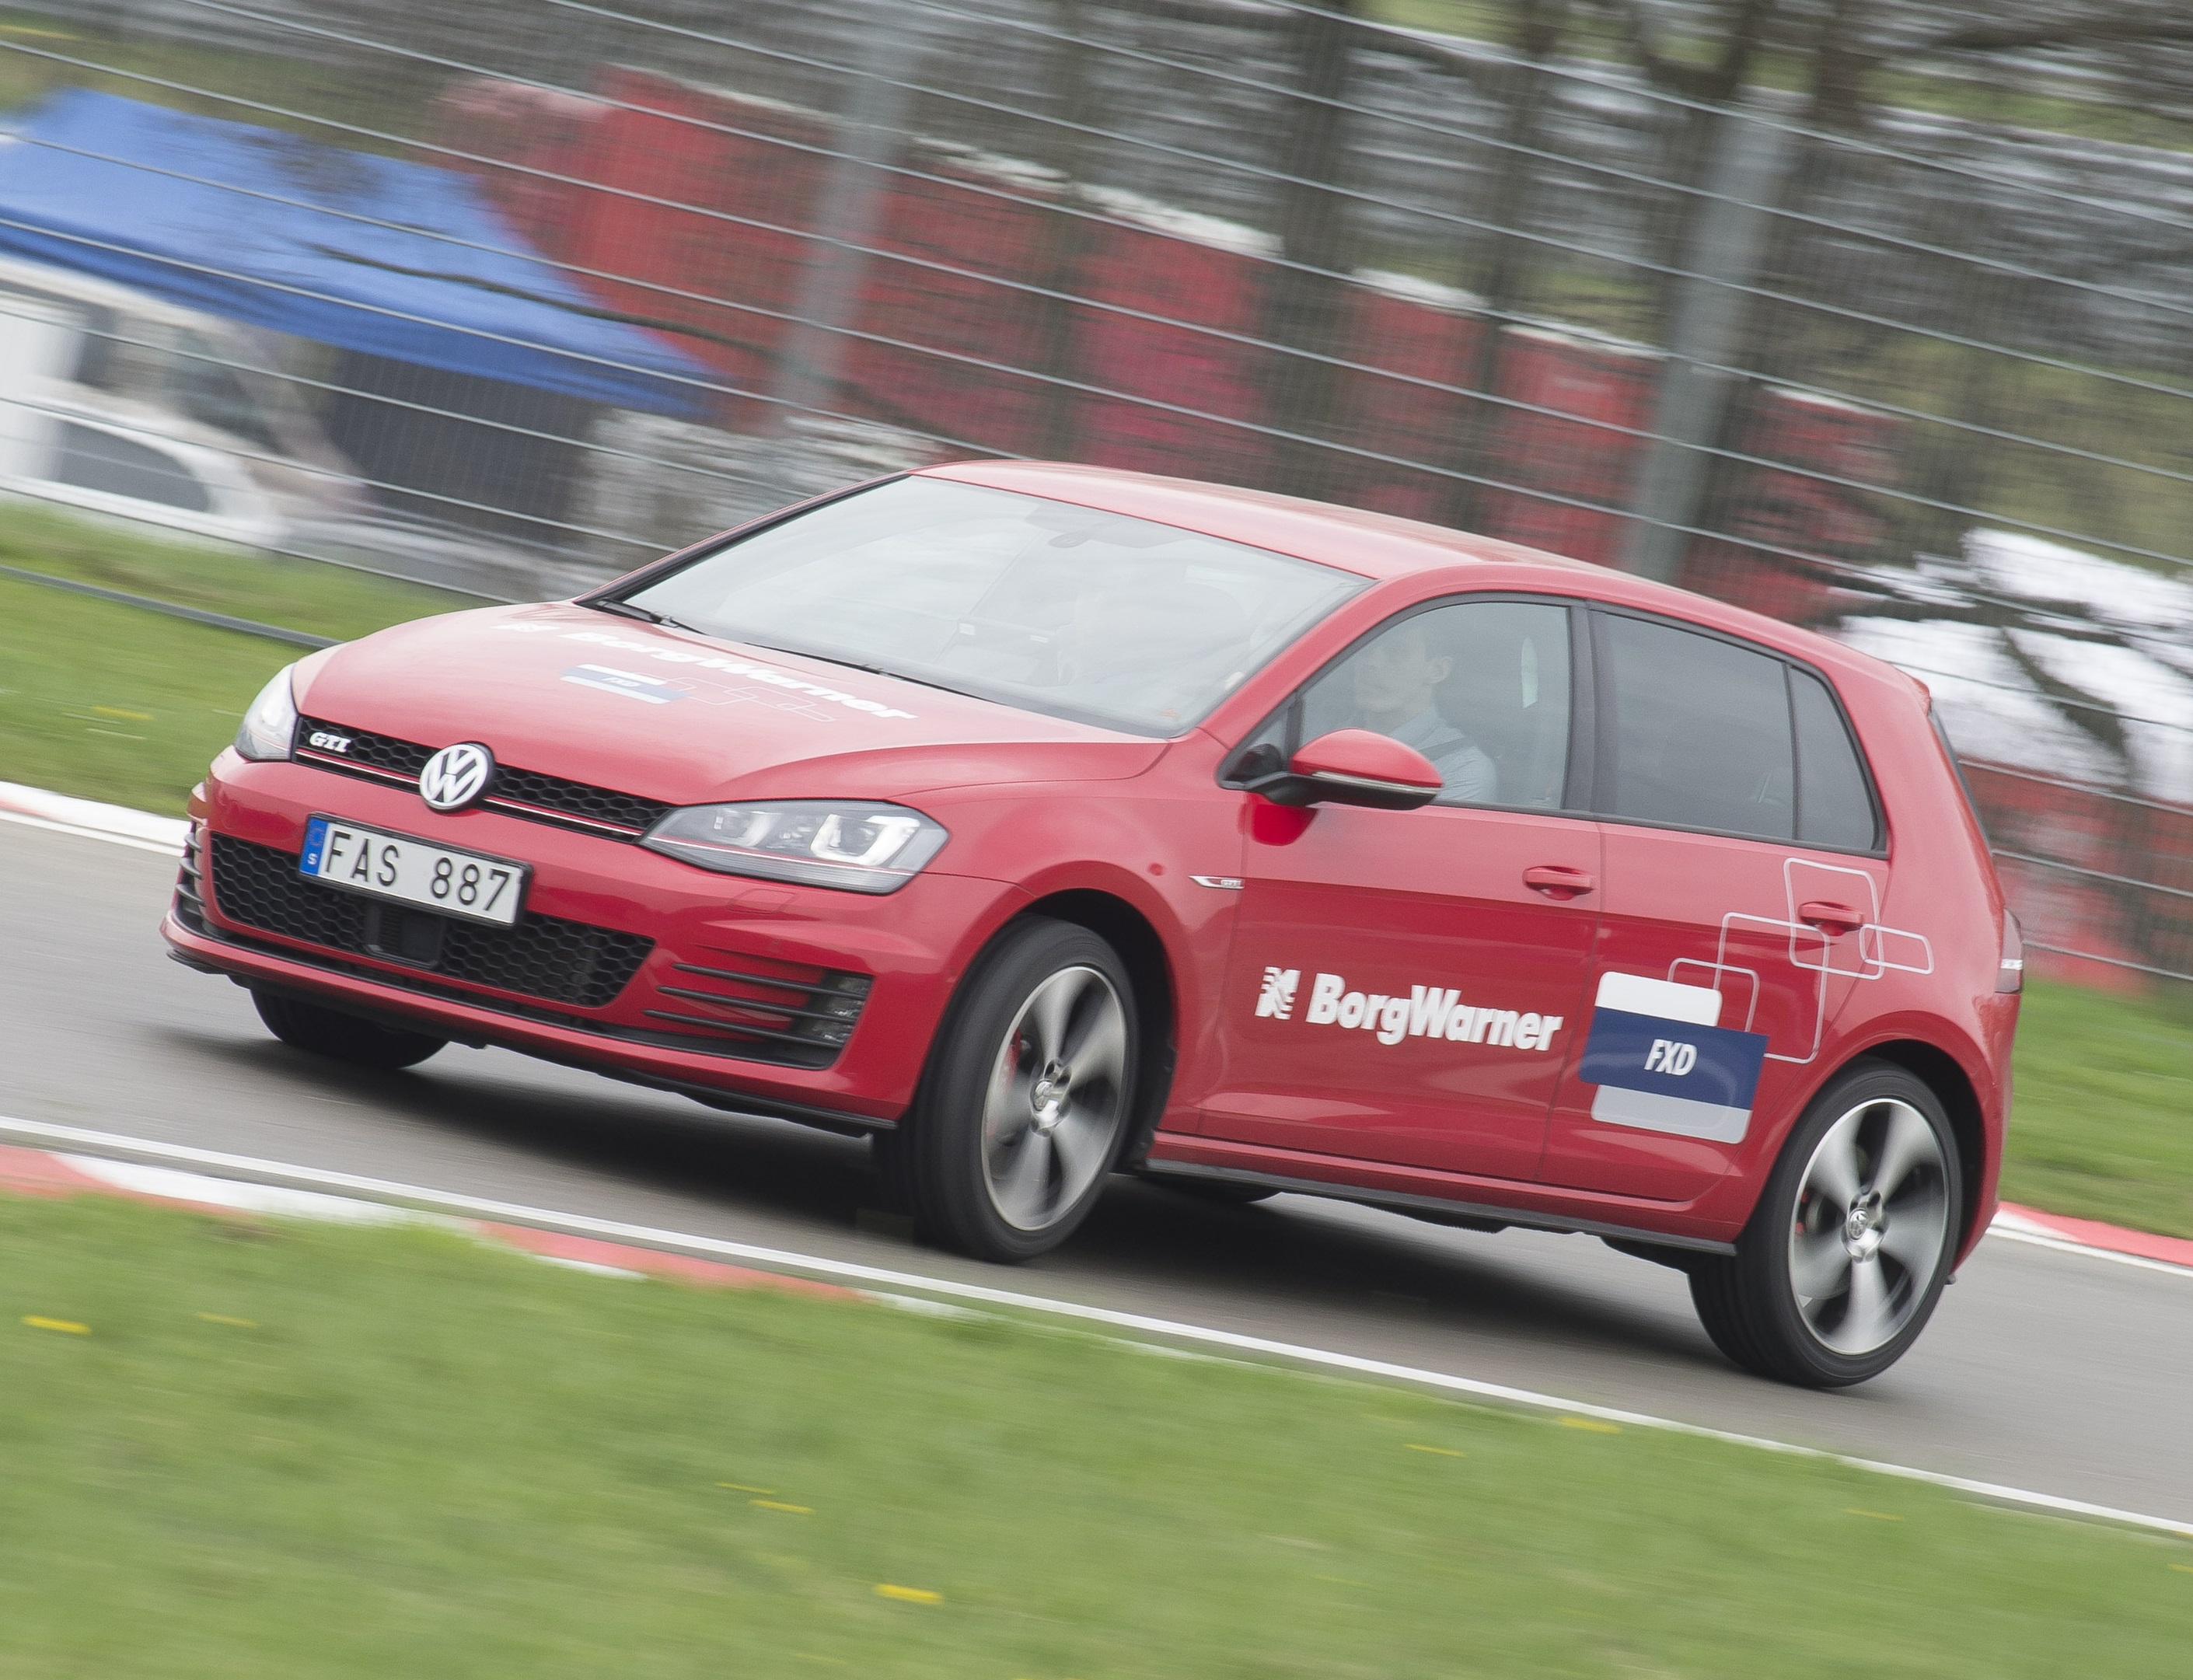
\includegraphics[width=1\textwidth]{Pictures/golf}
	\caption {Golf GTi Mk7 equipped with FXD.}
	\label{golf}
\end{figure}